\documentclass[conference]{IEEEtran}
\usepackage[main=portuguese,provide=*]{babel}
\usepackage{cite}
\usepackage{amsmath,amssymb,amsfonts}
\usepackage{graphicx}
\graphicspath{{output/}{../output/}{./}}
\usepackage{textcomp}
\usepackage{xcolor}
\usepackage[hidelinks]{hyperref}

\begin{document}

\title{Calibração de Câmera e Remoção de Distorção com OpenCV}

\author{
    \IEEEauthorblockN{
        \begin{tabular}{c}
            Gustavo Gabriel Ripka \\
            GRR20203935
        \end{tabular}
        \qquad \qquad
        \begin{tabular}{c}
            Arthur Barreto Godoi \\
            GRR20224377
        \end{tabular}
    }
    \vspace{0.2cm}
    \IEEEauthorblockA{
        \textit{Departamento de Informática} \\
        \textit{Universidade Federal do Paraná -- UFPR}\\
        Curitiba, Brasil
    }
}

\maketitle

\begin{abstract}
Este trabalho realiza a calibração de uma câmera de smartphone a partir de
fotografias de um tabuleiro quadriculado com quadrados de 9~cm. Foram
capturadas 52 imagens, das quais 33 foram consideradas válidas e
consistentes. Os cantos internos do tabuleiro (9$\times$4) foram detectados
com \texttt{findChessboardCorners} e refinados com precisão subpixel. A
calibração pelo método de Zhang forneceu a matriz intrínseca $K$ e os
coeficientes de distorção, com erro de reprojeção RMS de
$1{,}12$~px. A distorção foi removida das imagens e um experimento de
projeção 3D$\rightarrow$2D verificou que pontos no espaço 3D são
projetados nas coordenadas observadas com erro médio inferior a
$0{,}8$~px, inclusive em imagens não usadas no ajuste.
\end{abstract}

\begin{IEEEkeywords}
calibração de câmera, modelo pinhole, distorção de lente, OpenCV, método de Zhang.
\end{IEEEkeywords}

\section{Introdução}

A calibração de câmera estima os parâmetros que relacionam coordenadas
3D do mundo com coordenadas 2D na imagem. No modelo \emph{pinhole}, um
ponto $(X,Y,Z)$ é projetado em $(x,y)$ segundo
\begin{equation}
x = f_x \frac{X}{Z} + c_x, \qquad y = f_y \frac{Y}{Z} + c_y,
\end{equation}
o que, em coordenadas homogêneas, corresponde a
\begin{equation}
\begin{bmatrix} x \\ y \\ 1 \end{bmatrix}
\sim
\underbrace{\begin{bmatrix} f_x & s & c_x \\ 0 & f_y & c_y \\ 0 & 0 & 1 \end{bmatrix}}_{K}
\begin{bmatrix} R & t \end{bmatrix}
\begin{bmatrix} X \\ Y \\ Z \\ 1 \end{bmatrix}.
\end{equation}

A matriz $K$ reúne os parâmetros \emph{intrínsecos} (distâncias focais
$f_x,f_y$ em pixels, centro óptico $(c_x,c_y)$ e, opcionalmente, o
\emph{skew} $s$); a matriz $[R\,|\,t]$ reúne os parâmetros
\emph{extrínsecos} (posição e orientação da câmera). Lentes reais
introduzem distorção, modelada por
\begin{equation}
\begin{aligned}
x_d &= x\,(1 + k_1 r^2 + k_2 r^4 + k_3 r^6) + 2p_1 xy + p_2(r^2+2x^2),\\
y_d &= y\,(1 + k_1 r^2 + k_2 r^4 + k_3 r^6) + p_1(r^2+2y^2) + 2p_2 xy,
\end{aligned}
\end{equation}
com coeficientes radiais $k_1,k_2,k_3$ e tangenciais $p_1,p_2$, onde
$r^2 = x^2+y^2$.

O método de Zhang~\cite{zhang2000} calibra a câmera a partir de várias
vistas de um tabuleiro plano, dispensando alvos 3D dedicados. Neste
trabalho aplicamos esse método por meio da biblioteca
OpenCV~\cite{opencv}, seguindo os tutoriais de calibração da
ferramenta.

\section{Metodologia}

\subsection{Aquisição das imagens}

Foi utilizado um tabuleiro quadriculado com quadrados de
$9~\text{cm}\times 9~\text{cm}$ (alvo de $10\times5$ quadrados, ou seja,
$9\times4$ cantos internos). Foram capturadas 52 fotografias com a câmera
de um smartphone. As imagens foram distribuídas em duas resoluções; como
o OpenCV exige um único tamanho de imagem por calibração, adotou-se o
grupo dominante de $902\times1600$~px. Das imagens nesse formato, 33
apresentaram o tabuleiro detectado de forma completa e foram usadas.

\subsection{Detecção dos cantos}

Para cada imagem, os cantos internos foram localizados com
\texttt{cv2.findChessboardCorners} (com limiar adaptativo, normalização e
filtragem de quadriláteros) e refinados em precisão subpixel com
\texttt{cv2.cornerSubPix} (janela $11\times11$). A Figura~\ref{fig:det}
mostra um exemplo de detecção. O tamanho do padrão foi determinado
automaticamente, testando vários candidatos e escolhendo o que foi
detectado no maior número de imagens, o que confirmou $9\times4$ cantos.

\subsection{Calibração}

Com os pontos 3D do tabuleiro ($z=0$, passo de $0{,}09$~m) e os
respectivos pontos 2D, aplicou-se \texttt{cv2.calibrateCamera}, que
estima $K$, os coeficientes de distorção e a pose de cada vista
minimizando o erro de reprojeção. Optou-se pelo modelo de distorção de
quatro parâmetros $(k_1,k_2,p_1,p_2)$, fixando $k_3=0$: a inclusão de
$k_3$ praticamente não reduziu o erro (RMS $1{,}098$ vs.\ $1{,}122$~px)
mas tornou os coeficientes mal condicionados e introduziu distorção
inversa na correção, indicando \emph{overfitting} (as fotos foram
tomadas a distâncias semelhantes).

\begin{figure}[!t]
\centering
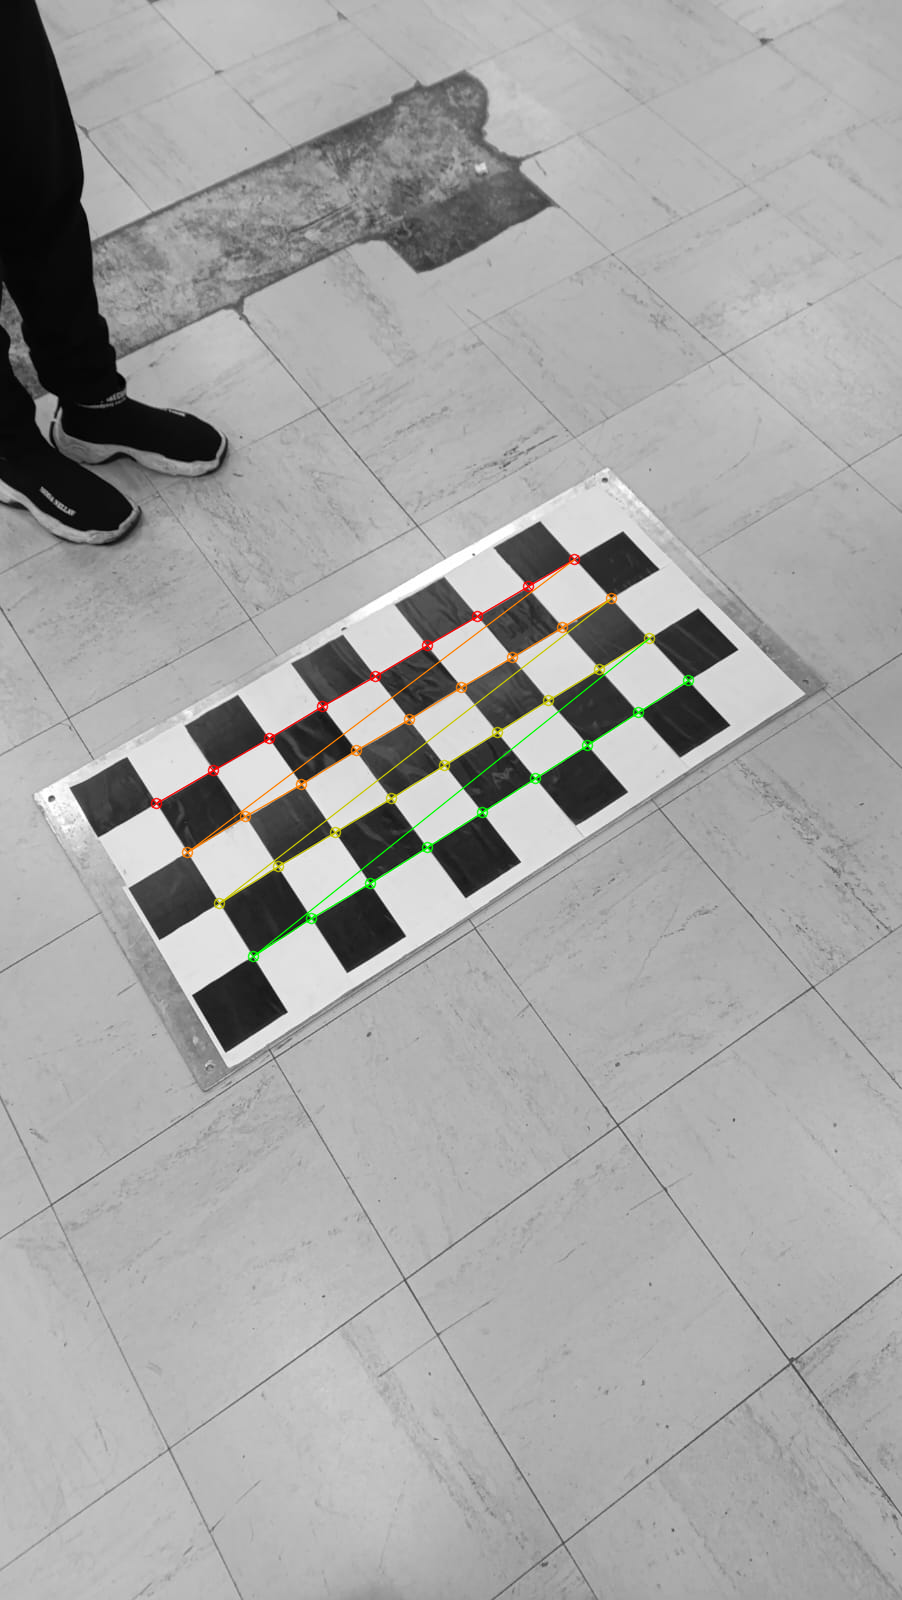
\includegraphics[width=\columnwidth]{deteccao_cantos.png}
\caption{Exemplo de detecção dos $9\times4$ cantos internos do tabuleiro
(em vermelho) em uma das imagens utilizadas.}
\label{fig:det}
\end{figure}

\section{Resultados}

A calibração resultou nos seguintes parâmetros:

\begin{equation}
K =
\begin{bmatrix}
1049{,}26 & 0 & 442{,}49 \\
0 & 1070{,}06 & 921{,}86 \\
0 & 0 & 1
\end{bmatrix},
\end{equation}
com coeficientes de distorção
\begin{equation}
(k_1,k_2,p_1,p_2) = (0{,}0062,\ 0{,}0971,\ 0{,}0042,\ -0{,}0033).
\end{equation}

O erro de reprojeção global (RMS) foi de $1{,}122$~px, com erro médio de
$0{,}783$~px e erro máximo de $3{,}27$~px por imagem. Os valores são
pequenos e compatíveis com uma calibração de boa qualidade para imagens
de celular (que já passam por compressão). Os coeficientes de distorção
são modestos, o que é esperado em câmeras de smartphone, cujo
\emph{pipeline} de imagem frequentemente já corrige parte da distorção
geométrica.

\subsection{Remoção de distorção}

A distorção foi removida com \texttt{cv2.undistort}, usando a nova
matriz de câmera ótima. A Figura~\ref{fig:undist} compara imagens
originais e corrigidas. Nas versões corrigidas, linhas do piso e das
paredes ficam retas, confirmando a remoção da distorção de barril.

\begin{figure}[!t]
\centering
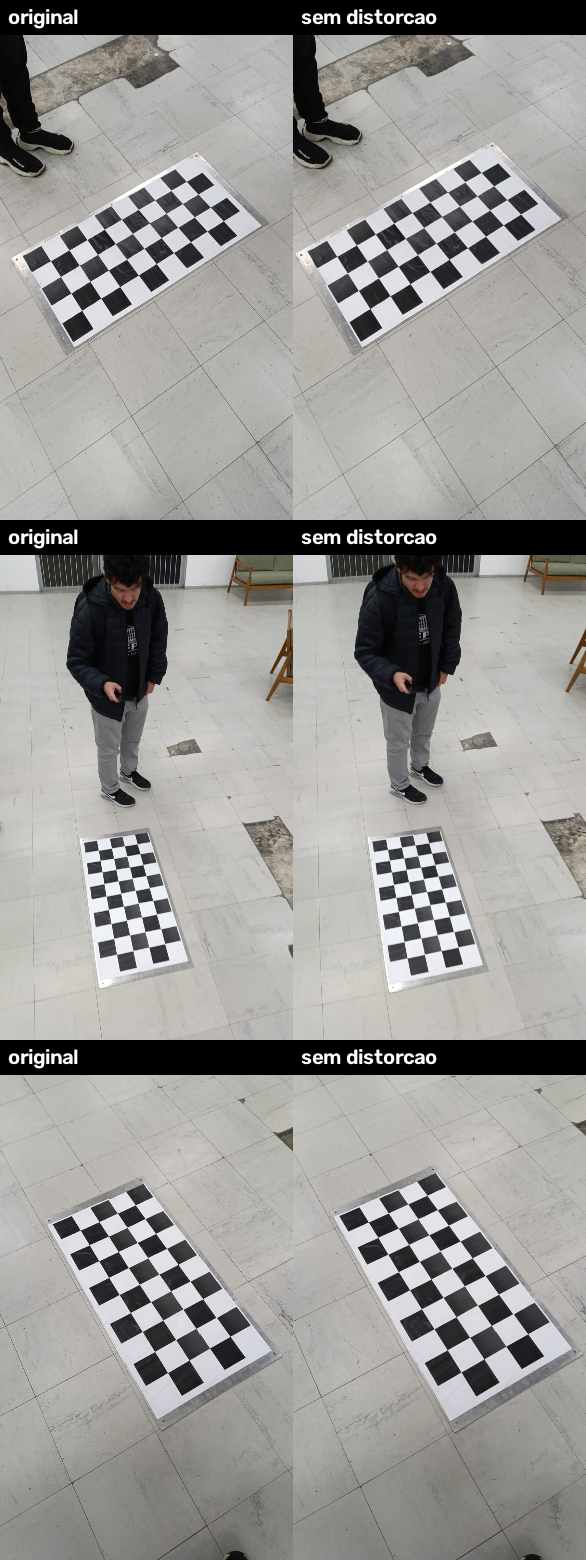
\includegraphics[height=0.78\textheight]{distorcao_antes_depois.png}
\caption{Remoção de distorção: à esquerda as imagens originais e à
direita as versões corrigidas (\emph{sem distorção}).}
\label{fig:undist}
\end{figure}

\section{Experimento 3D $\rightarrow$ 2D}

Para verificar a calibração, tomamos as posições 3D dos cantos do
tabuleiro e determinamos suas coordenadas nas imagens. Usando os
parâmetros calibrados e a pose obtida por \texttt{solvePnP}, os pontos
3D foram projetados com \texttt{projectPoints} e comparados com os
cantos efetivamente detectados.

Além da projeção direta, foi feito um teste de generalização
\emph{leave-one-out}: para cada imagem de teste, a câmera foi
recalibrada sem essa imagem e, em seguida, os pontos 3D foram projetados
nela. Isso confirma que a calibração prediz coordenadas em imagens que
não participaram do ajuste. A Tabela~\ref{tab:proj} resume os erros e a
Figura~\ref{fig:proj} mostra a sobreposição.

\begin{table}[!t]
\centering
\caption{Erro da projeção 3D$\rightarrow$2D (px). (A) projeção direta;
(B) \emph{leave-one-out}.}
\label{tab:proj}
\begin{tabular}{lcccc}
\hline
Imagem & (A) médio & (A) máx & (B) médio & (B) máx \\
\hline
img.\ 1 & 0,591 & 1,292 & 0,597 & 1,298 \\
img.\ 2 & 0,504 & 1,460 & 0,508 & 1,466 \\
img.\ 3 & 0,783 & 1,583 & 0,800 & 1,610 \\
\hline
\end{tabular}
\end{table}

Os erros médios são inferiores a $0{,}8$~px tanto na projeção direta
quanto no teste \emph{leave-one-out}, praticamente iguais entre si. Isso
mostra que a calibração é estável e que as coordenadas projetadas
coincidem com as observadas, mesmo em imagens novas.

\begin{figure*}[!t]
\centering
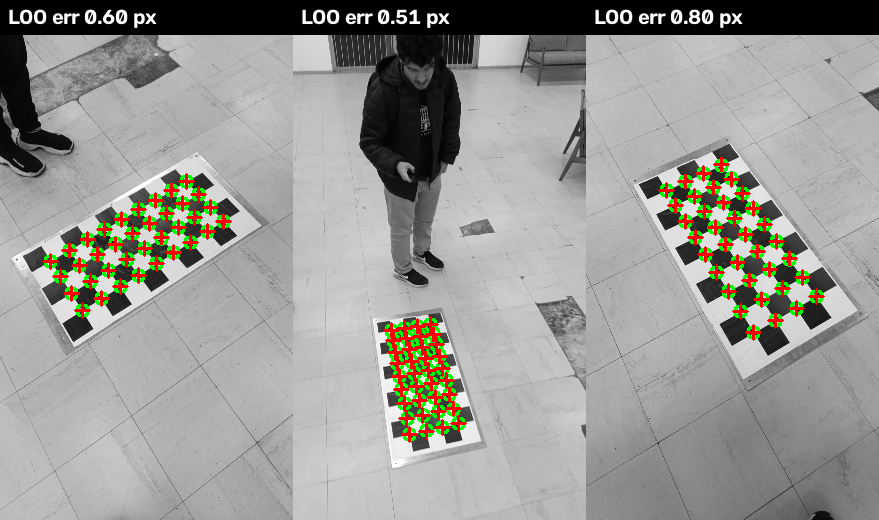
\includegraphics[width=0.9\textwidth]{projecao_3d2d.png}
\caption{Pontos 3D projetados (cruzes vermelhas) sobre os cantos
observados (círculos verdes) para três imagens, no teste
\emph{leave-one-out}. A sobreposição é praticamente exata.}
\label{fig:proj}
\end{figure*}

\section{Conclusão}

A calibração da câmera foi realizada com sucesso, fornecendo a matriz
intrínseca e os coeficientes de distorção, com RMS de $1{,}12$~px. A
remoção de distorção tornou retas as linhas da cena, e o experimento
3D$\rightarrow$2D confirmou que a câmera calibrada projeta pontos do
espaço 3D nas coordenadas corretas, inclusive em imagens não usadas no
ajuste (erro médio $<0{,}8$~px). A principal dificuldade foi a
quantidade de imagens descartadas (corte do tabuleiro, padrão não
detectado e resoluções distintas) e o condicionamento do modelo de
distorção, resolvido com um modelo de quatro parâmetros. Como trabalho
futuro, seria possível calibrar duas câmeras em configuração estéreo
para estimar a posição 3D de pontos presentes em ambas as imagens.

\section*{Repositório}

\url{https://github.com/gg-gustavo/cam-calibration}

\begin{thebibliography}{1}

\bibitem{zhang2000}
Z.~Zhang, ``A flexible new technique for camera calibration,''
\emph{IEEE Transactions on Pattern Analysis and Machine Intelligence},
vol.~22, no.~11, pp.~1330--1334, 2000.

\bibitem{opencv}
G.~Bradski, ``The OpenCV Library,'' \emph{Dr.\ Dobb's Journal of
Software Tools}, 2000.

\bibitem{hz}
R.~Hartley and A.~Zisserman, \emph{Multiple View Geometry in Computer
Vision}, 2nd ed. Cambridge University Press, 2004.

\end{thebibliography}

\end{document}
